\section{Case Study}
An example will be introduced to show how the heterogeneous multi-platform code generation based on IMCL model.


\subsection{The IMCL group model}

\begin{figure}[!htb]
  \centering
        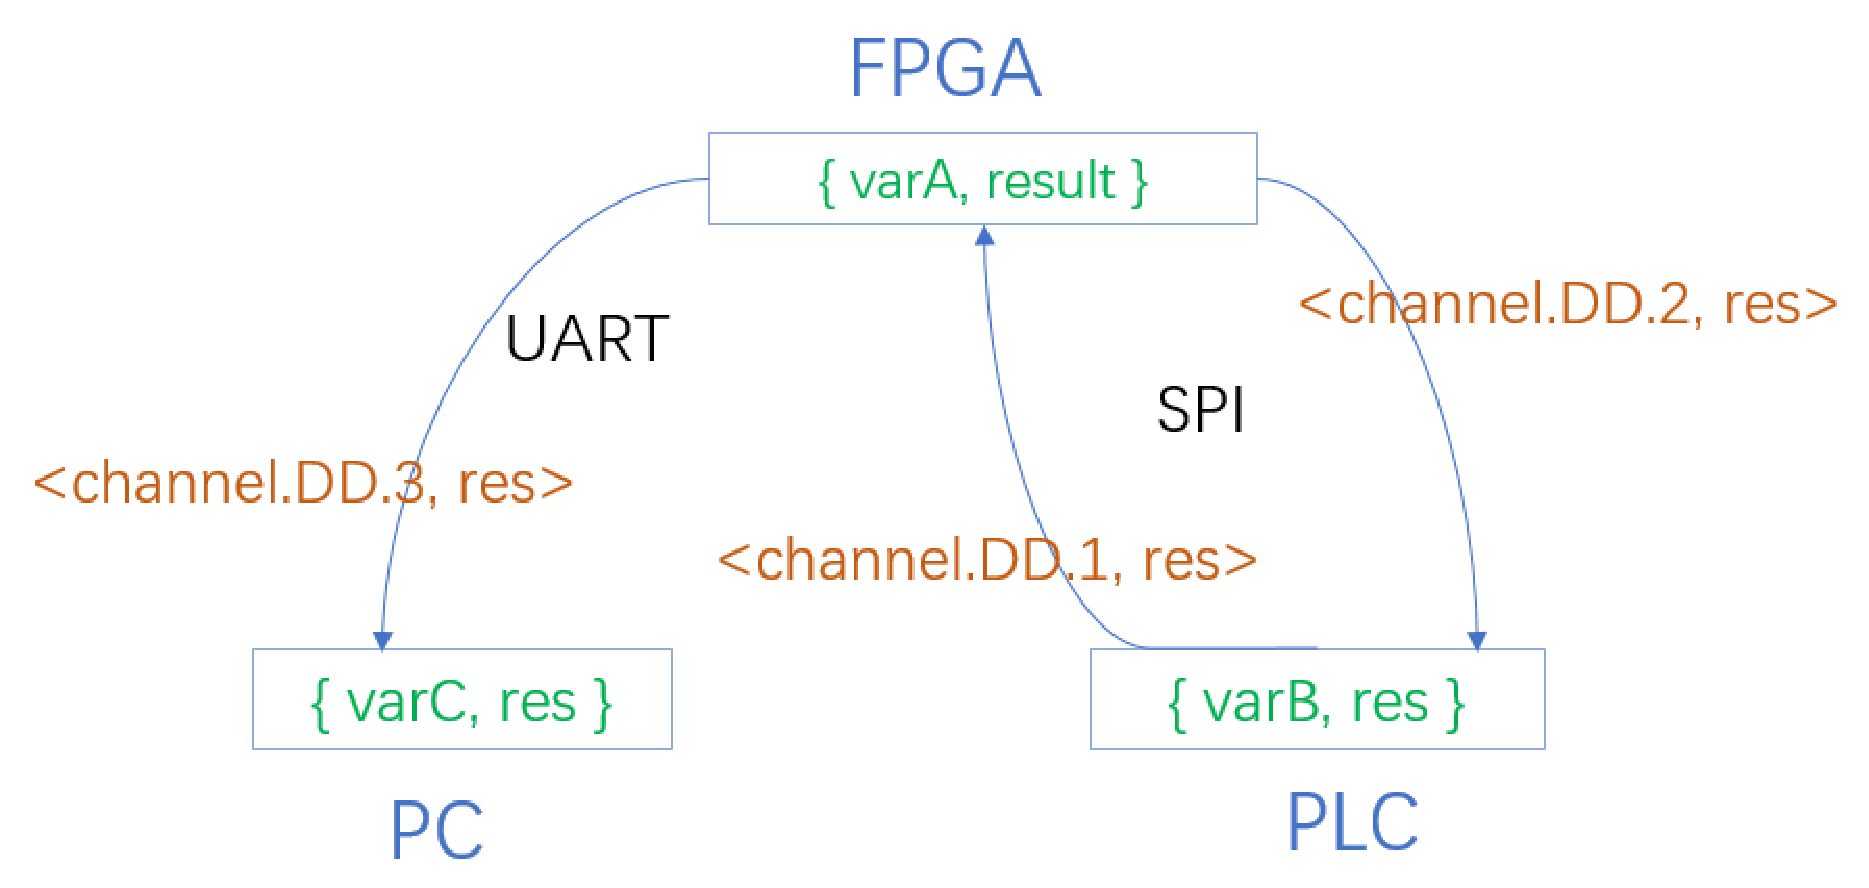
\includegraphics[height=1.5in, width=3.0in]{Compute_example}
  \caption{Heterogeneous computing systems of FPGA, PLC and PC}\label{Compute_example}
\end{figure}
The Fig \ref{Compute_example} is a computing system composed of three different platforms. Each of the three platforms, FPGA, PLC and PC, has its own independent computing and system control functions. Among them use SPI agreement between FPGA and PC, use UART agreement between FPGA and PLC. Each platform's program contains a set of specific variables, and they work together to achieve the ultimate computational task.

\begin{figure}[!tb]
  \centering
        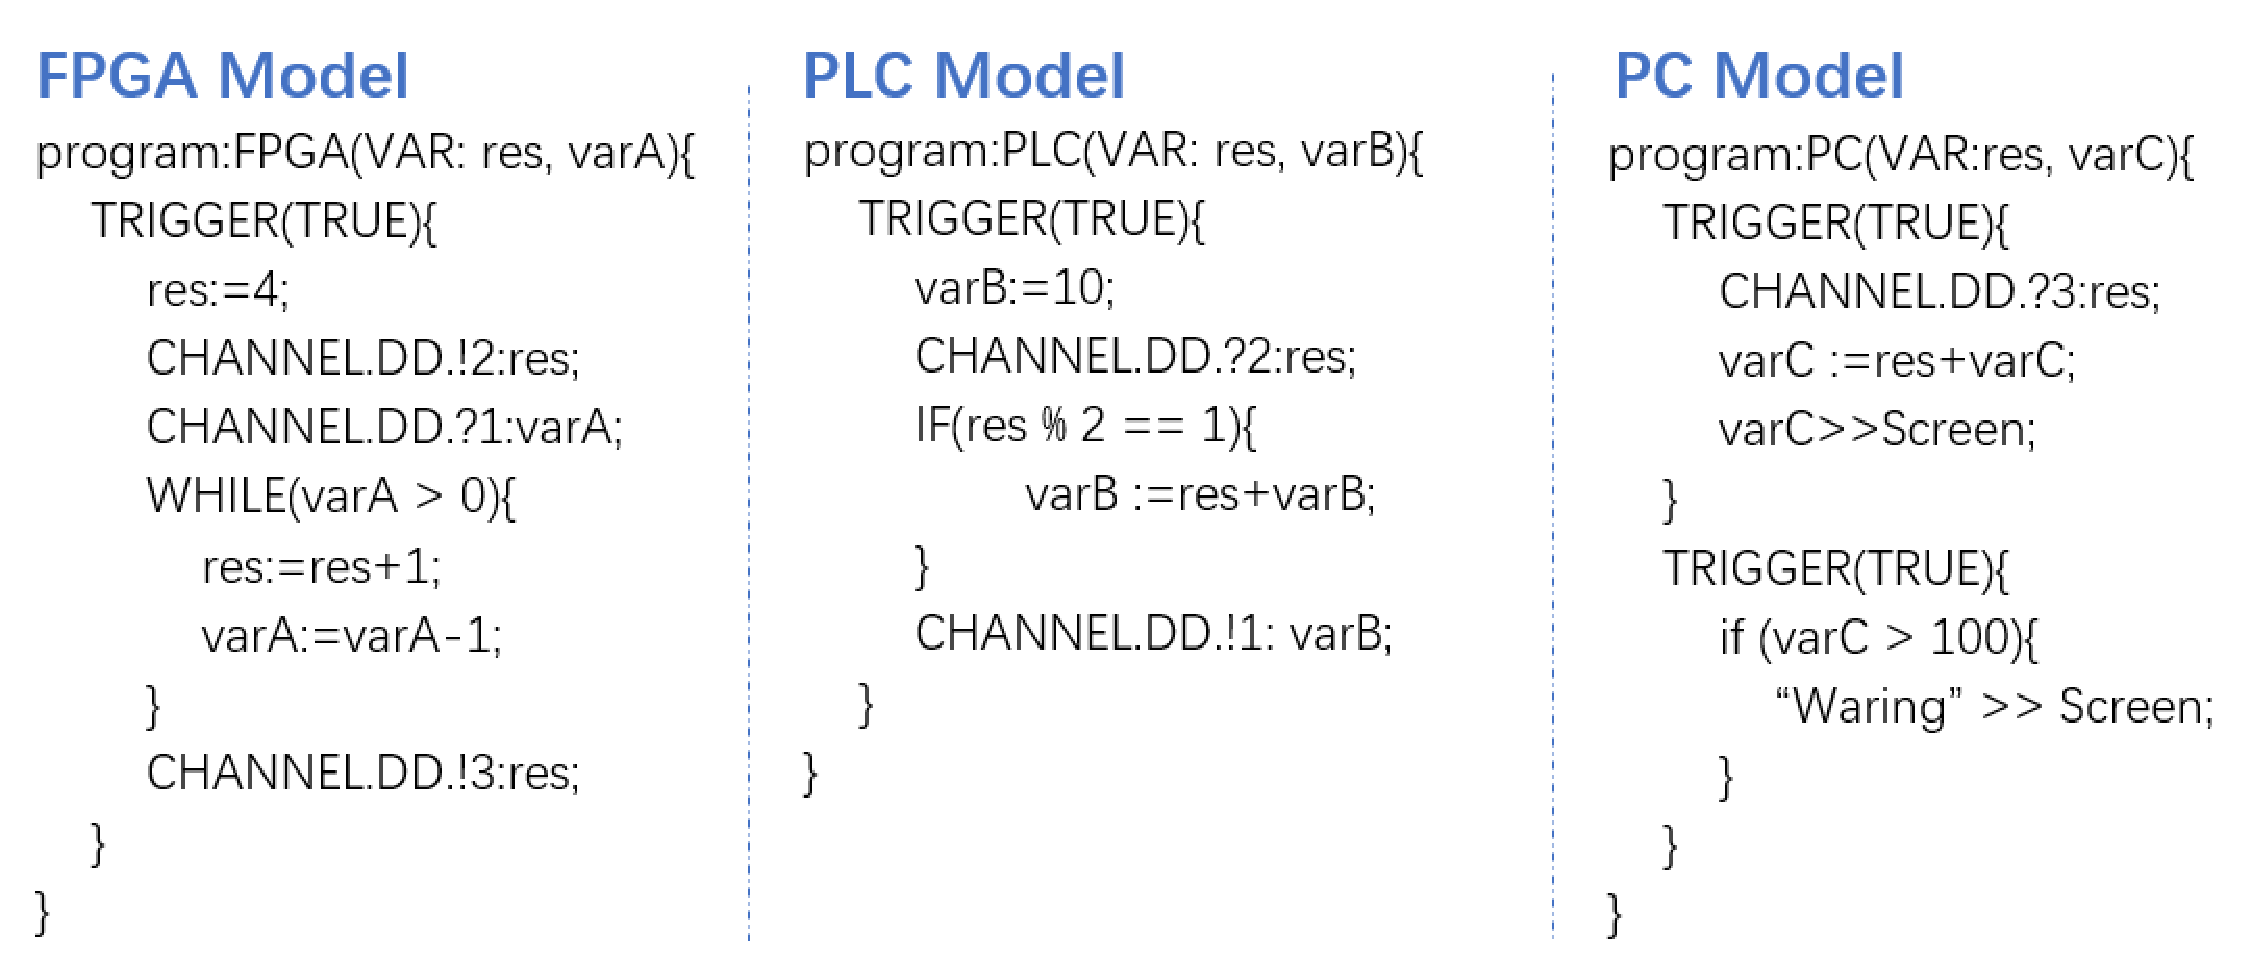
\includegraphics[height=1.8in, width=3.3in]{IMCL_group_models}
  \caption{IMCL group models of FPGA, PLC and PC}\label{group_models}
\end{figure}

\begin{figure}[!thb]
  \centering
        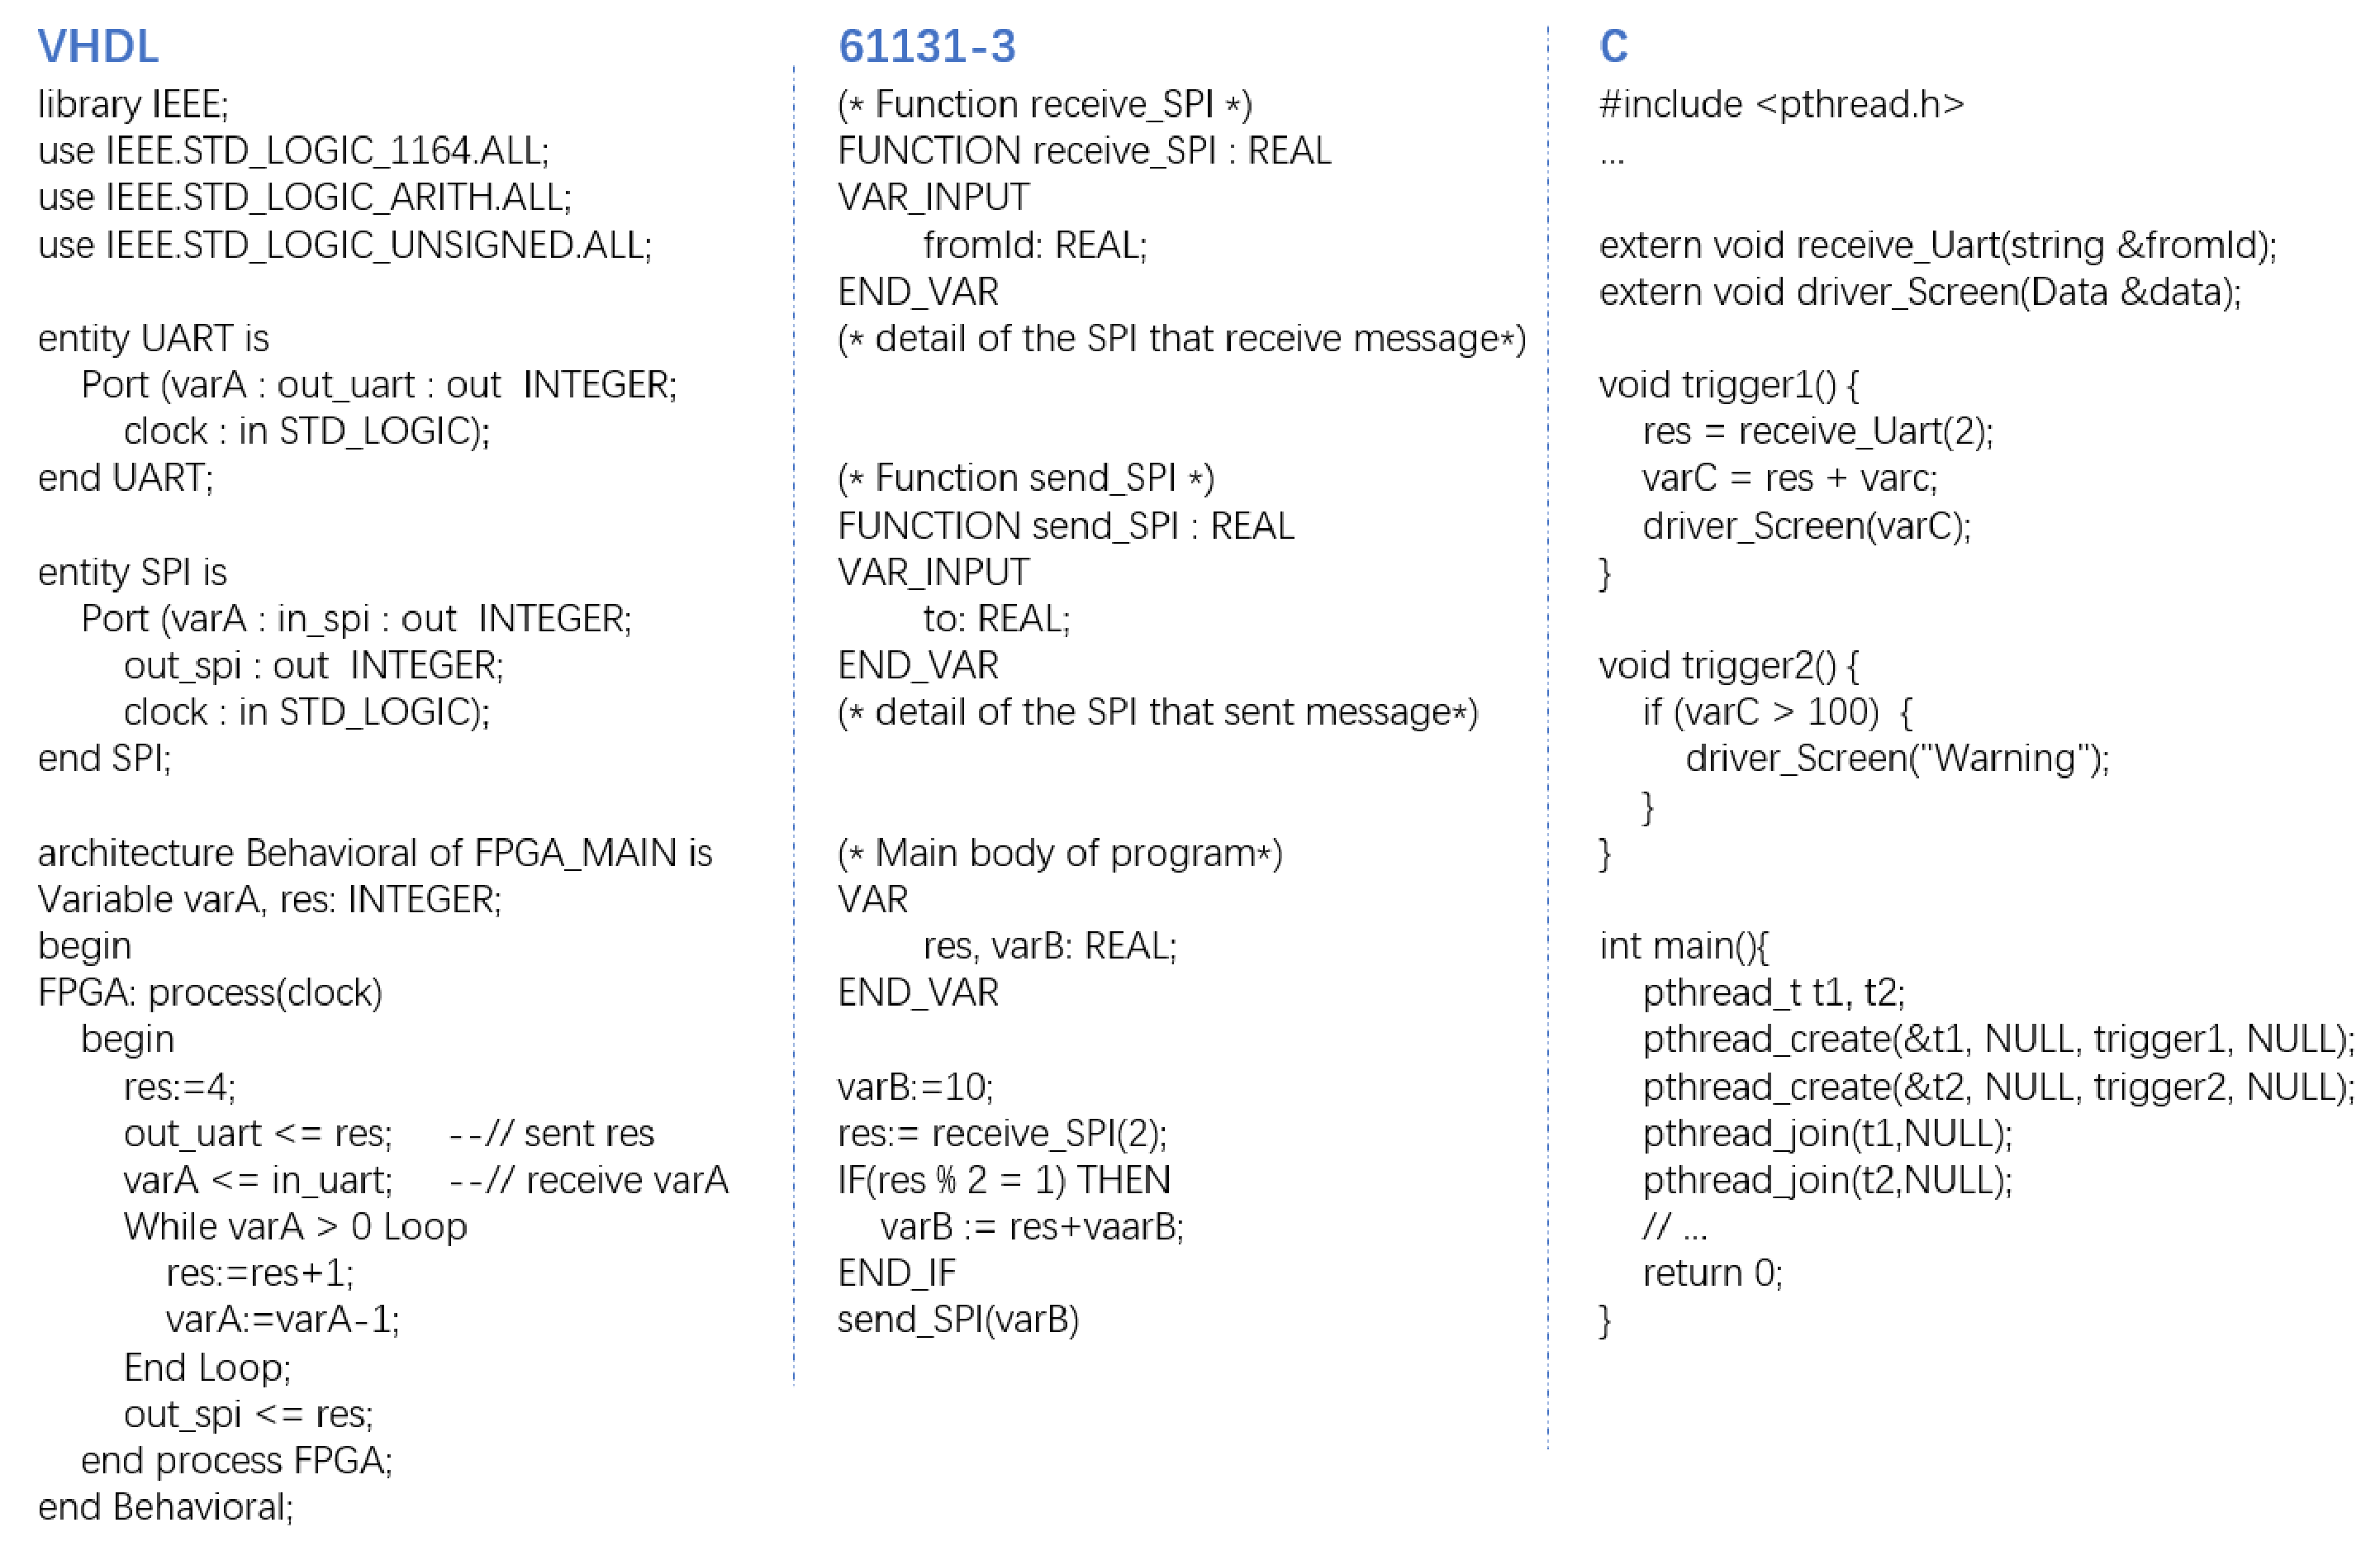
\includegraphics[height=2.0in, width=3.2in]{MultiPlatform_codes_generation}
  \caption{Heterogeneous Multi-platform Code Generation based on IMCL group models(VHDL, 61131-3 and C language)}\label{MultiPlatform_codes_generation}
\end{figure}


Firstly, we use IMCL to describe the entire system. The system model includes three IMCL models that correspond to FPGAs, PCs, and PLCs. Each model contains control functions such as logic operations and communications. The three models communicate data through communications to perform collaborative calculations. The entire system's IMCL model is shown in Fig \ref{group_models}.


\subsection{Multi-platform Code Generation based}


The above three platforms: FPGA, PLC, PC constitute a heterogeneous system. According to the defined five kinds of transformation rules, by analyzing the abstract syntax tree of the IMCL model program, the IMCL group model can finally generate the target platform code corresponding to the corresponding system.

The code in Fig \ref{MultiPlatform_codes_generation} shows the Heterogeneous Multi-platform Code generated by the defined approach. In the VHDL language, we use two Entity to define the communication protocol UART and SPI respectively, and use Behavior to define the function of the main body. In 61131-3, we define the communication function SPI through the functions receive\_SPI and send\_SPI, and use ST language to describe the system's function. In the C language, we implement the communication function by defining the receive\_Uart interface, and define the information scheduling relationship to the device Screen by defining the function driver\_Screen. Based on the analysis of the equivalence relationship between the three platforms and IMCL's system descriptions, we can conclude that our approach to approach code generation is feasible and has application value.
In future work, we will continue to study more efficient conversion methods, and we will explore the conversion rules between IMCL and more platforms. 